\clearpage
\thispagestyle{empty} 
\begin{center}
    \vspace*{\fill} 
    \Huge \textbf{Chapter 1} \\
    \Huge \textbf{Security Attacks}
    \vspace*{\fill}
\end{center}
\clearpage

\chapter{Security Attacks}

\section{Definitions and Key Concepts}
\begin{itemize}
    \item \textbf{Security Attack:} Any action compromising the security of information owned by an organization.\index{Security Attack@\hypertarget{SecurityAttack.ind}{\phantom{Security Attack}}\href{\#SecurityAttack.ind}{Security Attack}}
    \item \textbf{Security Mechanism:} A process or device designed to detect, prevent, or recover from a security attack.\index{Security Mechanism@\hypertarget{SecurityMechanism.ind}{\phantom{Security Mechanism}}\href{\#SecurityMechanism.ind}{Security Mechanism}}
    \item \textbf{Security Service:} A service that enhances the security of data processing systems and information transfers, countering security attacks using security mechanisms.\index{Security Service@\hypertarget{SecurityService.ind}{\phantom{Security Service}}\href{\#SecurityService.ind}{Security Service}}
\end{itemize}

\section{Threat vs. Attack}
\begin{itemize}
    \item \textbf{Threat:} Any circumstance or event with the potential to adversely impact organizational operations, assets, individuals, or the nation via unauthorized access, destruction, disclosure, modification of information, and/or denial of service.\index{Threat@\hypertarget{Threat.ind}{\phantom{Threat}}\href{\#Threat.ind}{Threat}}
    \item \textbf{Attack:} Any malicious activity attempting to collect, disrupt, deny, degrade, or destroy information system resources or the information itself.\index{Attack@\hypertarget{Attack.ind}{\phantom{Attack}}\href{\#Attack.ind}{Attack}}
\end{itemize}

\section{Types of Security Attacks}

\subsection{Passive Attacks}
\begin{itemize}
    \item \textbf{Nature:} Eavesdropping or monitoring transmissions without affecting system resources.\index{Passive Attack@\hypertarget{PassiveAttack.ind}{\phantom{Passive Attack}}\href{\#PassiveAttack.ind}{Passive Attack}}
    \item \textbf{Goals:} Obtain information being transmitted.\index{Eavesdropping@\hypertarget{Eavesdropping.ind}{\phantom{Eavesdropping}}\href{\#Eavesdropping.ind}{Eavesdropping}}
    \item \textbf{Types:}
    \begin{itemize}
        \item \textit{Release of Message Contents:} Eavesdropping on communications such as phone conversations, emails, or transferred files.\index{Release of Message Contents@\hypertarget{ReleaseContents.ind}{\phantom{Release of Message Contents}}\href{\#ReleaseContents.ind}{Release of Message Contents}}
        \item \textit{Traffic Analysis:} Observing the pattern of messages, frequency, and length without examining the contents.\index{Traffic Analysis@\hypertarget{TrafficAnalysis.ind}{\phantom{Traffic Analysis}}\href{\#TrafficAnalysis.ind}{Traffic Analysis}}
    \end{itemize}
    \item \textbf{Characteristics:} Difficult to detect; prevention usually involves encryption.\index{Encryption@\hypertarget{Encryption.ind}{\phantom{Encryption}}\href{\#Encryption.ind}{Encryption}}
\end{itemize}

\subsection{Active Attacks}
\begin{itemize}
    \item \textbf{Nature:} Involves modification of stored or transmitted data or the creation of false data.\index{Active Attack@\hypertarget{ActiveAttack.ind}{\phantom{Active Attack}}\href{\#ActiveAttack.ind}{Active Attack}}
    \item \textbf{Types:}
    \begin{itemize}
        \item \textit{Masquerade:} One entity pretends to be another, often combined with other active attacks.\index{Masquerade@\hypertarget{Masquerade.ind}{\phantom{Masquerade}}\href{\#Masquerade.ind}{Masquerade}}
        \item \textit{Replay:} Passive capture and retransmission of data to produce unauthorized effects.\index{Replay Attack@\hypertarget{ReplayAttack.ind}{\phantom{Replay Attack}}\href{\#ReplayAttack.ind}{Replay Attack}}
        \item \textit{Data Modification:} Alteration of legitimate messages or reordering/delaying them to produce unauthorized effects.\index{Data Modification@\hypertarget{DataModification.ind}{\phantom{Data Modification}}\href{\#DataModification.ind}{Data Modification}}
        \item \textit{Denial of Service:} Preventing or inhibiting normal use or management of communication facilities, either targeting specific entities or disrupting entire networks.\index{Denial of Service@\hypertarget{DenialOfService.ind}{\phantom{Denial of Service}}\href{\#DenialOfService.ind}{Denial of Service}}
    \end{itemize}
    \item \textbf{Characteristics:} Detection and recovery are primary goals since absolute prevention is difficult.\index{Detection@\hypertarget{Detection.ind}{\phantom{Detection}}\href{\#Detection.ind}{Detection}}\index{Recovery@\hypertarget{Recovery.ind}{\phantom{Recovery}}\href{\#Recovery.ind}{Recovery}}
\end{itemize}

\begin{figure}[h!]
    \centering
    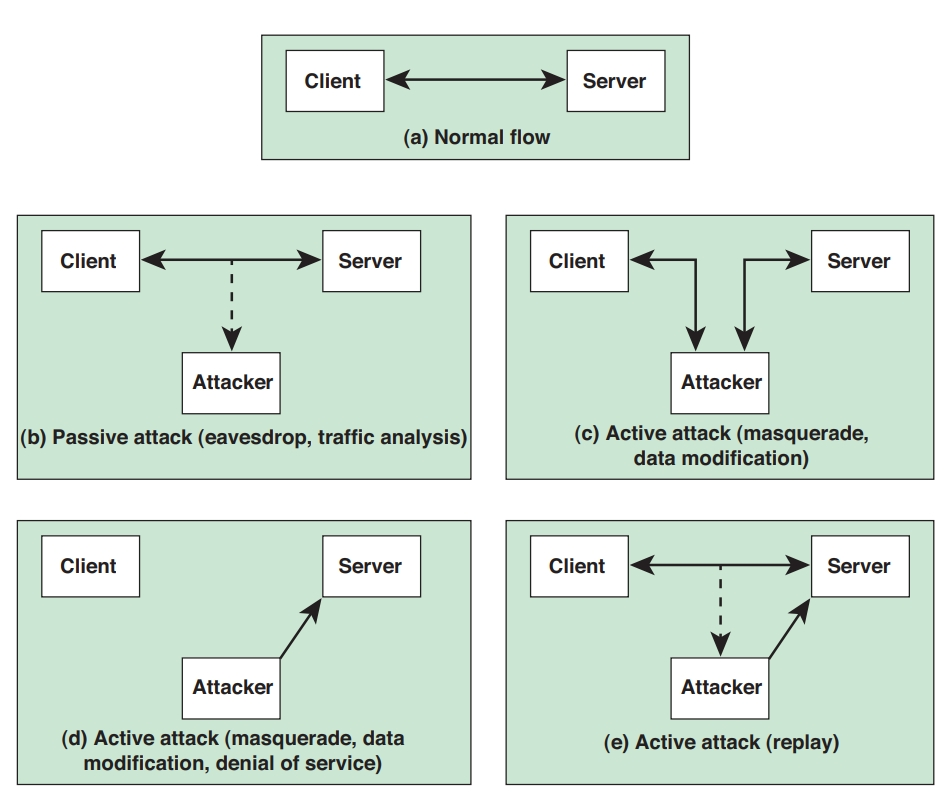
\includegraphics[width=\linewidth]{Data_Privacy_and_Cryptography/Figures/security_attacks.jpeg}
    \caption{Security Attacks}
    \label{fig:security_attacks}
\end{figure}

\section{Illustrations of Security Attacks}
\begin{itemize}
    \item \textbf{Passive Attack Example:} Eavesdropping on client-server communication without disturbing the flow.\index{Eavesdropping@\hypertarget{EavesdroppingExample.ind}{\phantom{Eavesdropping}}\href{\#EavesdroppingExample.ind}{Eavesdropping}}
    \item \textbf{Active Attack Examples:}
    \begin{itemize}
        \item \textit{Masquerade:} Man-in-the-middle attack, intercepting and pretending to be the client or server.\index{Man-in-the-middle Attack@\hypertarget{ManInTheMiddle.ind}{\phantom{Man-in-the-middle Attack}}\href{\#ManInTheMiddle.ind}{Man-in-the-middle Attack}}
        \item \textit{Data Modification:} Selectively modifying data communicated between client and server.\index{Data Modification@\hypertarget{DataModificationExample.ind}{\phantom{Data Modification}}\href{\#DataModificationExample.ind}{Data Modification}}
        \item \textit{Replay:} Capturing and reusing client messages.\index{Replay Attack@\hypertarget{ReplayExample.ind}{\phantom{Replay Attack}}\href{\#ReplayExample.ind}{Replay Attack}}
        \item \textit{Denial of Service:} Flooding the server with data or triggering resource-consuming actions.\index{Denial of Service@\hypertarget{DenialExample.ind}{\phantom{Denial of Service}}\href{\#DenialExample.ind}{Denial of Service}}
    \end{itemize}
\end{itemize}
In Figure \ref{fig:security_attacks}, you can see the visual illustration of security attacks.